%----------------------------------------------------------------------------------------
%	PACKAGES AND OTHER DOCUMENT CONFIGURATIONS
%----------------------------------------------------------------------------------------

\documentclass[a4paper,12pt]{article} % Default font size is 12pt, it can be changed here

% Packages:
\usepackage{geometry} % Required to change the page size to A4
\usepackage{graphicx,xcolor} %colors and images
\usepackage{subfigure} %useful for multiple figures in one float
\usepackage{float} % Allows putting an [H] in \begin{figure} to specify the exact location of the figure
\usepackage{amsmath, amssymb} %Mathematical symbols
\usepackage[exponent-product=\cdot, per-mode=symbol]{siunitx} %Useful for physical quantities with units
\usepackage[notrig]{physics} %contains all kinds of useful abbreviations for braket, derivatives, etc.
\usepackage{enumitem,fancyhdr,lastpage,parskip} %For item lists, for headers and footers and no indents
\usepackage[numbers,square,super,sort&compress]{natbib} %For a bibliography
\usepackage{listings} %Listings package is for scripts
\usepackage{cprotect} %For verbatim code in title...
%\usepackage{cite}
\usepackage[colorlinks,linkcolor=blue]{hyperref}
\usepackage{subcaption}
\usepackage{wrapfig}
\allowdisplaybreaks



% CODE ENVIRONMENT
\definecolor{mygreen}{rgb}{0,0.6,0} \definecolor{mygray}{rgb}{0.5,0.5,0.5} \definecolor{mymauve}{rgb}{0.58,0,0.82}
\lstset{ 
  backgroundcolor=\color{white},   % choose the background color; you must add \usepackage{color} or \usepackage{xcolor}; should come as last argument
  basicstyle=\footnotesize,        % the size of the fonts that are used for the code
  breakatwhitespace=true,          % sets if automatic breaks should only happen at whitespace
  breaklines=true,                 % sets automatic line breaking
  linewidth=\linewidth,            % sets the linewidth of the code frame to the linewidth of the document
  %commentstyle=\color{gray}\itshape, % make comments gray and italic 
  captionpos=b,                    % sets the caption-position to bottom
  deletekeywords={...},            % if you want to delete keywords from the given language
  escapeinside={\%*}{*)},          % if you want to add LaTeX within your code
  extendedchars=true,              % lets you use non-ASCII characters; for 8-bits encodings only, does not work with UTF-8
  firstnumber=1,                   % start line enumeration with line 1000
  frame=single,	                   % adds a frame around the code
  keepspaces=true,                 % keeps spaces in text, useful for keeping indentation of code (possibly needs columns=flexible)
  language=Python,                 % the language of the code
  morekeywords={as, self, Dict, Tuple, List, Any, Union, None, ...},            % if you want to add more keywords to the set
  numbers=left,                    % where to put the line-numbers; possible values are (none, left, right)
  numberstyle=\tiny,               % line numbers are smaller
  numbersep=5pt,                   % how far the line-numbers are from the code
  keywordstyle=\color{blue},
  commentstyle=\color{mygreen},
  rulecolor=\color{black},         % if not set, the frame-color may be changed on line-breaks within not-black text (e.g. comments (green here))
  showspaces=false,                % show spaces everywhere adding particular underscores; it overrides 'showstringspaces'
  showstringspaces=false,          % underline spaces within strings only
  stringstyle=\color{mymauve}, 
  %stringstyle=\color{gray},        % strings are also gray
  showtabs=false,                  % show tabs within strings adding particular underscores
  stepnumber=1,                    % the step between two line-numbers. If it's 1, each line will be numbered
  tabsize=2,	                   % sets default tabsize to 2 spaces
  title=\lstname,                  % show the filename of files included with \lstinputlisting; also try caption instead of title
}
%\lstset{basicstyle=\footnotesize, breakatwhitespace=false, breaklines=true, commentstyle=\color{mygreen}, extendedchars=true, frame=single, keepspaces=true, keywordstyle=\color{blue}, language=Python, numbers=left,                    numbersep=5pt, numberstyle=\tiny\color{mygray},  rulecolor=\color{black}, showspaces=false, showstringspaces=false, showtabs=false, stringstyle=\color{mymauve}, tabsize=3, title=\lstname, captionpos=b}
%See for comments for instance here: https://tex.stackexchange.com/questions/83882/how-to-highlight-python-syntax-in-latex-listings-lstinputlistings-command

%%% SET HEADER/FOOTER
\pagestyle{fancy}
\fancyhf{}
\fancyhead[C]{\nouppercase{\leftmark}} 
\cfoot{\thepage\ of \pageref*{LastPage}}

\begin{document}

%----------------------------------------------------------------------------------------
%	TITLE PAGE
%----------------------------------------------------------------------------------------

\begin{titlepage}

\newcommand{\HRule}{\rule{\linewidth}{0.5mm}} % Defines a new command for the horizontal lines, change thickness here

\center % Center everything on the page
\begin{figure}[H] \center{
\includegraphics[width=0.2\linewidth]{logo}} \end{figure}
\textsc{\LARGE Universiteit Leiden}\\[1.5cm] % Name of your university/college
\textsc{\Large Computational Physics}\\[0.5cm] % Major heading such as course name


\HRule \\[0.4cm]
{ \huge \bfseries Molecular dynamics simulation of Argon atoms}\\[0.4cm] % Title of your document
\HRule \\[1.5cm]

\begin{minipage}{0.45\textwidth}
\begin{flushleft} \large
\emph{Students:}\\
Davey \textsc{Plugers} \small{(\texttt{s2946661})}\\
\large Zhen \textsc{Xiang} \small{(\texttt{s2731126})} % Your name
\end{flushleft}
\end{minipage}
\begin{minipage}{0.4\textwidth}
\begin{flushright} \large
\emph{Lecturers:} \\
\large Matthieu \textsc{Schaller}\\ % Supervisor's Name
\hspace{1cm} \\
\end{flushright}
\end{minipage}\\[4cm]

{\large \today\\Leiden}\\[3cm] % Date, change the \today to a set date if you want to be precise

\vfill % Fill the rest of the page with whitespace

\end{titlepage}

%----------------------------------------------------------------------------------------
%	Abstract
%----------------------------------------------------------------------------------------

\begin{abstract}
This report is mainly based on Molecular dynamics using the Verlet algorithm and minimum image convention. This is used to simulate 108 Argon atoms with a Face-centered cubic(FCC) structure interacting through a Lennard-Jones potential. The resulting pair correlation functions are in agreement with known theoretical and experimental results. The pressures measured in this simulation are:\\ 
\begin{center}
    

$\rho = 1.2, T=0.5 \Rightarrow P_{Solid} = 8.60 \pm 0.02$\\
$\rho = 0.8, T=1.0 \Rightarrow P_{Liquid} = 1.02 \pm 0.02$\\
$\rho = 0.3, T=3.0 \Rightarrow P_{Gas} = 0.96 \pm 0.01$\\.
\end{center}
\par
All code is publicly available on  \href{https://github.com/boson112358/cmp-project}{our github page}
\end{abstract}
\newpage
%----------------------------------------------------------------------------------------
%	TABLE OF CONTENTS
%----------------------------------------------------------------------------------------
\vspace{2em}
\setcounter{tocdepth}{2} %toc doesn't show subsubsections
\tableofcontents % Include a table of contents

\newpage % Begins the essay on a new page instead of on the same page as the table of contents


\setlength{\parskip}{1em}

%----------------------------------------------------------------------------------------
%	INTRODUCTION
%----------------------------------------------------------------------------------------
\newpage
\section{Introduction} % Major section
Molecular dynamics(MD) is a wildly used molecular simulation methods. The method mainly relies on Newtonian mechanics to simulate the motion of a molecular system to extract samples from a system composed of different states of the molecular system, thereby calculating the configuration of the system as it develops a period of time. Based on the result of the configuration, the thermodynamic quantities and other macroscopic properties of the system are further calculated. Molecular dynamics simulation is a common method in modern science, which can study the physical and chemical properties of molecules, molecular reaction processes, etc. In recent decades, it has been widely used in chemical physics\cite{suleimanov2011bimolecular}, biophysics\cite{vsponer2007molecular}\cite{lague2004pressure},material physics\cite{novko2015ab} and many other fields.\par
Argon is the colorless and odorless gas at room temperature and is the third-most abundant gas in the Earth's atmosphere.Therefore, its properties have been extensively studied. Our goal is to use molecular dynamics simulation to simulate the three states of argon atoms, solid, liquid, and gas and obtain observable in different phases.Use temperature and density as initial conditions to calculate the pressure and pair correlation function of argon atoms in different phases.\par
This report is organised as follow. Section \ref{Theoretical Background} describes the theoretical background of Verlet algorithm and molecular dynamics simulation of Argon and its properties. The methods is presented in Section \ref{Methods}, we mainly use Verlet algorithm to calculate force and velocity of each time step and use dimensionless expression to remove the units in our simulation. Section \ref{Results} shows the results of our simulation, it demonstrates the pair correlation function and pressure of each phase of argon, and Section \ref{Summary} summarises our findings.\par

%----------------------------------------------------------------------------------------
%	THEORY
%----------------------------------------------------------------------------------------
\newpage
\section{Theoretical Background}
\label{Theoretical Background}
\subsection{Molecular Dynamics of Argon}
Molecular dynamics(MD) simulation\cite{braun2019best} plays an important role to understand and predict the properties of researched system. MD simulations can solve the equation of motion of a system by using Newtonian Mechanics. Thus, we consider the motion of each particles is governed by Newton's second law:
\begin{equation}\label{motion}
    m\frac{\mathrm{d}^{2} \boldsymbol{x}}{\mathrm{d} t^{2}} = \boldsymbol{F}(\boldsymbol{x}) = -\nabla U(\boldsymbol{x})
\end{equation}
For multi-particle system, the force act on each particle becomes:
\begin{equation}
    \boldsymbol{F}_i = \boldsymbol{F}(\boldsymbol{x}_i) = -\sum_{j} \nabla U(\boldsymbol{x}_i - \boldsymbol{x}_j)
\end{equation}
Our simulation is focused on a system with 108 Argon atoms in a three-dimensional box. Argon is a noble inert gas. Argon atoms are electrically neutral and will not generate Coulomb force when interacting with each other. When looking into nucleus and electron cloud, it exists attractive and compulsive interaction. So we can use Lennard-Jones potential\cite{jones1924determination}\cite{jones1924determination2} to describe the potential energy of each Argon atom. 
\begin{equation}\label{LJPot}
    U_{L-J}(r) = 4\epsilon \left[ \left(\frac{\sigma}{r}\right)^{12} - \left(\frac{\sigma}{r}\right)^{6}\right]
\end{equation}\par
The Lennard-Jones potential is a relatively simple mathematical model used to simulate the potential energy of the interaction between two electrically neutral molecules or atoms.It is used to describe the interaction between noble gas molecules with particular precision.\par
In a physical sense, the first term$1/r^{12}$can be considered to correspond to the role of two bodies repelling each other at a close distance, and the second term$1/r^6$ corresponds to the role of two bodies attracting(E.g. through van der Waals force) each other at a long distance.\par
The corresponding two-body force of the Lennard-Jones potential is:
\begin{equation}
    \boldsymbol{F}(\boldsymbol{x}) = 4\epsilon(12\frac{\sigma^{12}}{r^{13}}-6\frac{\sigma^6}{r^7})\frac{\boldsymbol{x}}{r}
\end{equation}
So for multi-particle system, the force becomes:
\begin{equation}
    \boldsymbol{F}(\boldsymbol{x}_i) =\sum_{j} 4\epsilon(12\frac{\sigma^{12}}{r^{13}}-6\frac{\sigma^6}{r^7})\frac{(\boldsymbol{x}_i-\boldsymbol{x}_j)}{r}
\end{equation}\par
For argon, the parameters is $\sigma/k_B = 119.8K$, and $\epsilon = 3.405 \mathring{A}$, and in our simulation we choose $\sigma/k_B = 100K$.\par
\subsection{Verlet algorithm}
Verlet algorithm\cite{verlet1967} is one of the most common integration methods in Newtonian mechanics, and it is widely used in the fields of Molecular Dynamics Simulation, planetary motion and fabric deformation simulation. The problem to be solved by the Verlet algorithm is that given the position $r$ and velocity $v$ of the particle at time $t$, get the position $r(t+dt)$ and velocity $v(t+dt)$ at time $t+dt$.\par
Verlet algorithm derived from \eqref{motion} using Taylor expansion:
\begin{equation}\label{v1}
    \boldsymbol{x}(t+h) = \boldsymbol{x}(t) + h\dot{\boldsymbol{x}}(t) + \frac{h^2}{2}\ddot{\boldsymbol{x}}(t) + \frac{h^3}{6}\dddot{\boldsymbol{x}}(t) + \mathcal{O}(h^4)
\end{equation}
\begin{equation}\label{v2}
    \boldsymbol{x}(t-h) = \boldsymbol{x}(t) - h\dot{\boldsymbol{x}}(t) + \frac{h^2}{2}\ddot{\boldsymbol{x}}(t) - \frac{h^3}{6}\dddot{\boldsymbol{x}}(t) + \mathcal{O}(h^4)
\end{equation}
Combining \eqref{motion}, \eqref{v1} and \eqref{v2} and \eqref{motion}, we obtain,
\begin{equation}
    \boldsymbol{x}(t+h) = 2\boldsymbol{x}(t) - \boldsymbol{x}(t-h) + \frac{h^2}{m}\boldsymbol{F}(\boldsymbol{x}(t)) + \mathcal{O}(h^4)
\end{equation}
So for the velocity we can obtain,
\begin{equation}
    \boldsymbol{v}(t) = \frac{\boldsymbol{x}(t+h)-\boldsymbol{x}(t-h)}{2h} + \mathcal{O}(h^2)
\end{equation}
Instead of using the algorithm above we change it into velocities directly. We use Taylor expansion for $\boldsymbol{v}$ and $\boldsymbol{\dot{v}}$,
\begin{equation}\label{velocity1}
    \boldsymbol{v}(t+h) = \boldsymbol{v}(t) + h\boldsymbol{\dot{v}}(t) + \frac{h^2}{2}\boldsymbol{\ddot{v}}(t) + \mathcal{O}(h^3)
\end{equation}
\begin{equation}\label{velocity2}
    \boldsymbol{\dot{v}}(t+h) = \boldsymbol{\dot{v}}(t) + h\boldsymbol{\ddot{v}}(t) + \mathcal{O}(h^2)
\end{equation}
Combining \eqref{velocity1} and \eqref{velocity2}, we obtain,
\begin{equation}\label{VVA1}
    \boldsymbol{v}(t+h) = \boldsymbol{v}(t) + \frac{h}{2m}(\boldsymbol{F}(\boldsymbol{x}(t+h)) - \boldsymbol{F}(\boldsymbol{x}(t))) + \mathcal{O}(h^3)
\end{equation}
We rewrite the \eqref{v1},
\begin{equation}\label{VVA2}
    \boldsymbol{x}(t+h) = \boldsymbol{x}(t) + h\boldsymbol{v}(t) + \frac{h^2}{2m}\boldsymbol{F}(\boldsymbol{x}(t)) + \mathcal{O}(h^3)
\end{equation}
So \eqref{VVA1} and \eqref{VVA2} is called velocity Verlet algorithm, we mainly use this algorithm to calculate motion of Argon atoms in our simulation.\par
\subsection{Minimum Image Convention}
In order to simulate a small scale system without creating hard borders and boundary conditions, it's possible to make use of the minimum image convention. This will generate periodic copies of the current simulation box. The particles in the original simulation will then be able to interact with either another real particle or the copied version of that particle.\cite{braun2019best}
\subsection{Velocity rescaling}
When initialising the conditions for the simulation all the velocity's will be distributed according to the following Gaussian Distribution:
\begin{equation}
    p(v_i) \sim exp{ (-mv^2_i)/(2k_BT)}
\end{equation}
These values are chosen according to the equipartition theorem such that we have.
\begin{equation}
    v_{equi}= \sqrt{3k_bT/m}
\end{equation}
However because of interactions with the potential it is possible that the average velocity of the system will change. This causes the system to act like it is at a higher temperature than originally intended.\\
\\
In reality this would not happen due to the law of increased multiplicity or more generally the second law of thermodynamics. This causes deviations from the mean to be reduced almost exponentially with respect to the amount of particles. \cite{Pearson}.\\
\\
Because in reality this would not be the cases it is important to periodically rescale all velocities such that the system is brought back to the desired temperature.
\begin{equation}
\begin{gathered}
 v_i \Rightarrow \lambda v_i \ \ \lambda = \sqrt{\frac{(N-1)3k_BT}{m\sum_iv^2_i}} \\
    E_{kin} = \sum_i \frac{m(\lambda v_i)^2}{2}  =\frac{(N-1)3k_bT}{2} = \frac{(N-1)mv^2_{equi}}{2} = E_{target}
\end{gathered}
\end{equation}
Calculating this $\lambda$ and multiplying all velocities will then make sure the system is being simulated at the right temperature again. 



\subsection{Pair Correlation Function}
The Pair Correlation Function is a function that scales according to the probability of finding a second particle quantisation at a distance r with respect to the original particle.\cite{Biology}.
This means it's a function that helps understand how the environment of a particle looks like in the simulation.\cite{chandler}\par
To calculate this one has to calculate the distance between all particle pairs up to a desired distance. These values can then be used to fill in a histogram n(r) which is averaged out over multiple configurations. The Pair Correlation Function is then defined the following way.
\begin{equation}\label{PairCorr}
    g(r) = \frac{2V}{N(N-1)}\frac{<n(r)>}{4\pi r^2\Delta r}
\end{equation}
Where the extra coefficients are defined to normalise the system's density in such a way that g(r) = 1 for a gas in the region outside of the first atom's coordination shell. In simpler terms, this means our average density with respect to the distance to a particle does not change.\cite{chandler} A good way to compare this with is the Pair Correlation Function of a solid, this will not be g(r) since the density will be distance dependent due to the strict lattice structure quantising the positions where atoms can move.

\subsection{Pressure}
It is possible to find an expression the Pressure in the system by using the Clausius Virial Theorem.\cite{verlet1967}\cite{Lion_2012}
\begin{equation}
    W^{tot}(\Vec{r}_1,...,\Vec{r}_N) = \sum_{i=1}^{N} \Vec{r}_i\cdot F^{tot}_i  
\end{equation}
Averaging this out over a 3 dimensional trajectory this becomes.
\begin{equation}
    < W^{tot}> = -3Nk_BT
\end{equation}
However $W^{tot}$ can be rewritten into $W^{Int} + W^{ext}$ where $W^{ext}$ is an expression dependent on the pressure of the system. Filling in this $W^{ext}$ for a 3-dimensional cube with one corner at the origin one can rewrite it to.
\begin{equation}
    <W^{ext}> =  <\sum_{i=1}^{3} \Vec{r}_i\cdot F^{ext}_i>, F^{ext}_i = -PL^2 \ \ \Rightarrow \ \ <W^{ext}> = -3PV
\end{equation}
Then $W^{int}$ can be expressed in function of the potential.
\begin{equation}
    <W^{int}> = \left<\frac{1}{2}\sum_i \sum_{j>i} r_{ij}\frac{\partial V(r_{ij})}{\partial r_{ij}}\right>
\end{equation}
Rewriting in function of P and inserting all values then gives a formula for the pressure.
\begin{equation}\label{Pressure}
    P = \frac{Nk_BT}{V} + \frac{1}{6V}\left< \sum_{i}\sum_{j>i} r_{ij}\frac{\partial V(r_{ij})}{\partial r_{ij}}\right>
\end{equation}
\newpage
\section{Methods}
\label{Methods}
\subsection{Dimensionless Expression}
While the potential defined by equation \eqref{LJPot} works fine to get results, it's not that convenient to use. Instead one can define dimensionless units to remove the $\epsilon$ and $\sigma$ from the equations. This has the added benefit that values will be closer to unity to prevent rounding errors and having the same magnitude for everything.\par
This can be done by rescaling the position and potential energy and then inserting these rescaled versions into other equations to get a dimensionless expression. We also define a dimensionless temperature since this will later be used to remove the Boltzmann constant from some equations.
\begin{equation}
\label{Rescale1}
\begin{array}{cc} \Tilde{x} = x/\sigma \ \ \  & \Tilde{V}(\Tilde{r}) = V(\Tilde{r})/\epsilon = 4[\Tilde{r}^{-12} - {\Tilde{r}^{-6}}] \\ \end{array} \ \ \ \Tilde{T} = \frac{Tk_B}{\epsilon}
\end{equation}
Then filling this in for acceleration one can define a new time step.
\begin{equation}
\begin{gathered}
    \frac{1}{\tau^2}\frac{d^2\Tilde{x}}{d\Tilde{t}^2}= \frac{1}{\sigma}\frac{d^2x}{dt^2} = -\frac{1}{m\sigma}\nabla V(r) = -\frac{\epsilon}{m\sigma}\nabla \Tilde{V}(\Tilde{r}) = - \frac{\epsilon}{m\sigma^2}\Tilde{\nabla}\Tilde{V}(\Tilde{r})\\
    \Tilde{t} = t/\sqrt{\frac{m\sigma^2}{\epsilon}}
\end{gathered}    
\end{equation}
And then yet again we use this to redefine the velocity and find expression for kinetic energy.
\begin{equation}
\begin{gathered}
    \Tilde{v} =  \frac{\Tilde{x}}{\Tilde{t}} = \sqrt{\frac{\sigma^2m}{\sigma^2\epsilon}} \frac{x}{t} = v\sqrt{\frac{m}{\epsilon}}\\
    E_{kin} = 0.5mv^2 = \epsilon * 0.5\Tilde{v}^2 = \epsilon * \Tilde{E}_{kin}
\end{gathered}    
\end{equation}
In this system, with $T=1K$, the particles move a typical distance of order $\sigma$ in time $\sqrt{m{\sigma}^2/\epsilon}$. And our time-step $h$ should be of order $10^{-3}$ to $10^{-2}$. So in our simulation, we choose the final time to be 10 time units and time-step is $10^{-3}$, our total steps is $1\times10^4$. The kinetic energy is in units of $\epsilon$ just like the potential in \eqref{Rescale1}. Now we shall use these dimensionless expressions to rewrite: The Maxwellian velocity distribution, the velocity rescaling factor, density, pair correlation function and the pressure.
\begin{equation*}
\begin{gathered}
    p(\Tilde{v}_i) \sim exp\left( \frac{-\Tilde{v}_i}{2\Tilde{T}}\right) \ i\in [x,y,z] \ \ \ \Tilde{\lambda} = \sqrt{\frac{(N-1)3\Tilde{T}}{\sum^N_j\Tilde{v}^2_j}} \ \ \ \Tilde{\rho} = \rho\sigma^3
    \end{gathered}
    \end{equation*}
    \begin{equation}
    \begin{gathered}
    \Tilde{g}(\Tilde{r}) \sim \frac{\Tilde{V}}{\Tilde{r}^2\Delta\Tilde{r}} = \frac{\sigma^3}{\sigma^3}\frac{V}{r^2\Delta r} \sim g(r)\\
    \end{gathered}
    \end{equation}
    \begin{equation*}
    \begin{gathered}
    \frac{P\sigma^3}{\epsilon} = \Tilde{T}\Tilde{\rho} - \frac{\Tilde{\rho}}{6N\epsilon}*\left<\sum_i\sum_{j>i} \frac{\sigma\epsilon}{\sigma}\frac{\Tilde{r}_{ij}\partial\Tilde{U}(\Tilde{r}_{ij})}{\partial\Tilde{r}}\right> =
    \Tilde{T}\Tilde{\rho} - \frac{\Tilde{\rho}}{6N}*\left<\sum_i\sum_{j>i} \frac{\Tilde{r}_{ij}\partial\Tilde{U}(\Tilde{r}_{ij})}{\partial\Tilde{r}}\right> = \Tilde{P}
\end{gathered}
\end{equation*}
Take note that the average of the  histogram values $n(r)$ which is normally used for the pair correlation function g(r) does not produce a scale factor. \par
\subsection{Verlet algorithm}
The implementation of the Verlet algorithm is done through a force function and the main code applying the dynamics to all the particles.
\small
\begin{lstlisting}
ForcePrevious = [np.array(TotalForce(k, 0)) for k in range(ParticleAmount)]
for tstep in bar:
    for j in range(ParticleAmount):
        Particles[j, 0] = Particles[j, 0] + Particles[j, 1] * TimeStepLength + TimeStepLength ** 2 / (2) * ForcePrevious[j]
        Particles[j, 0] = Particles[j, 0] % BoxSize
    for j in range(ParticleAmount):
        NewForce = TotalForce(j, -1)
        Particles[j, 1] = Particles[j, 1] + TimeStepLength / (2) * (NewForce + ForcePrevious[j])
        ForcePrevious[j] = NewForce
\end{lstlisting}
\normalsize
Line 4 and 5 update the positions and line 8 updates the velocities. To reduce computation the previous force value is saved and used again on the next iteration, this is done through line 1 for the first step and 9 for all the following steps.
\subsubsection{TotalForce Function}
This is a function that takes two inputs, the particle index: j, and the time step which has a special case structure and returns a force vector felt by the corresponding particle. The TotalForce function is able to access all previously saved particle positions allowing it for a much more general usage.\par
While this general case is no longer in use due to saving the previous force, it has been decided to leave this in for potential future usage. However it also has a special case for tstep==-1, by inserting this value it will use the not yet saved position in the Particles[j,0] array instead.\par
\subsubsection{Optimisation possibilities}
There are 2 main and very obvious optimisations possible. First off exploiting the symmetry of the force. In TotalForce the force vector of all particle pairs with j are added together. However by saving these,if TotalForce would be called for particle i we would already have the force due to the i and j interaction by multiplying it with -1. This would half computation at the cost of some memory.\par
The second optimisation would be to introduce broadcasting for numpy arrays. This would get rid of for loops and allow for much faster code. However due to a lack of time and experience it was not yet implemented.
\subsection{Pair correlation}
Calculation of the Pair Correlation is done by periodically calling the Histogram(Bins) function during the simulation. Subsequent calls add the histograms together and after the simulation the average is taken by dividing by the amount of calls. These values will then be inserted into formula \eqref{PairCorr} and this is then plotted.
\small
\begin{lstlisting}
def Histogram(Bins):
    Histo = np.histogram([BoxSize], bins=[BoxSize / (2 * Bins) * x for x in range(Bins + 1)])[0]
    for i in range(ParticleAmount):
        Distances = [DistancePoints(Particles[1 + i + j, 0], Particles[i, 0]) for j in range(ParticleAmount - i - 1)]
        Histo += np.histogram(Distances, bins=[BoxSize / (2 * Bins) * x for x in range(Bins +1)])[0]
    return Histo
\end{lstlisting}
\normalsize
Line 2 premakes an empty histogram with the desired binsize. Line 3 and 4 are then used to create an array consisting of all the current distances of particle pairs and 5 will then convert all of this into a histogram.
\subsection{Pressure}
To calculate the pressure a very specific value has to be calculated. The average of the sum of all the distance times force pairs (as denoted in formula \eqref{Pressure}). This sum is calculated multiple times during the simulation through the function SumDistTimesForce(). Afterwards it is averaged out and then used to calculate the pressure.\par
\newpage
\small
\begin{lstlisting}
def SumDistTimesForce():
    DistTimesForce = 0
    for i in range(ParticleAmount):
        for j in range(ParticleAmount - i - 1):
            Dist = DistancePoints(Particles[1 + i + j, 0], Particles[i, 0])
            DistTimesForce += (12 * (-2 / Dist ** 12 + 1 / Dist ** 6))
    return DistTimesForce

\end{lstlisting}
\normalsize
\newpage
\section{Results}
\label{Results}
\subsection{Verification of Validity}
While writing some code and blindly trusting the results would make coding a lot quicker to do. It's still a good idea to make sure your results correspond with known theoretical and experimental values. Because of this there will be multiple validations to make sure the code works as intended. In this subsection we talk about these methods and that our system is indeed valid.
\subsubsection{2-dimensional Animation}
Looking at the 2-dimensional animation is the most straightforward way to check some very important basic properties: Attraction from far away, repulsion when nearby, particles being mirrored when crossing the border and particles interacting with the nearest periodic copies of each other. Trying to show this effect with individual frames is quite hard however the code has the option to make a 2d animation. It is however recommended to check this using a 2d simulation and not a 3d since particles will overlap on the same z position.
\subsubsection{Total Energy Conservation}
Energy conservation is a very important requirement to have a physical system. It also helps to make sure there isn't an issue with the dimensions when converting force or energy into velocity. When plotting the total energy we should see a constant function that only jumps whenever the kinetic energy gets rescaled.\\
\begin{figure}[!h]
\centering
\begin{minipage}{.5\textwidth}
  \centering
  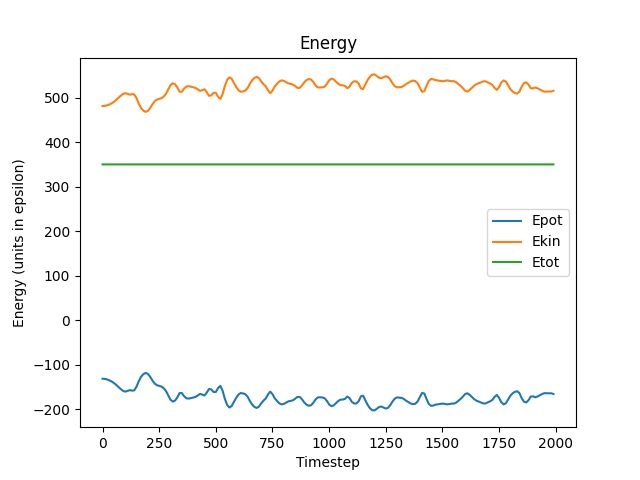
\includegraphics[width=0.95\linewidth]{Data/energy.png}
\end{minipage}%
\begin{minipage}{.5\textwidth}
  \centering
  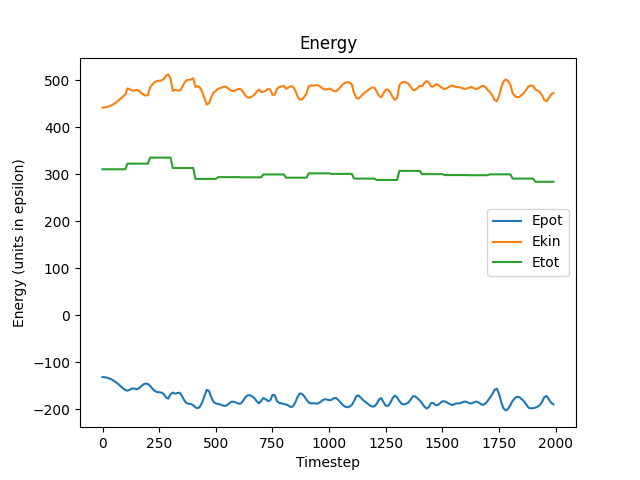
\includegraphics[width=0.95\linewidth]{Data/energyrescale.png}

\end{minipage}
\caption{Left: Energy plots for a system without rescaling. Right: Energy plots for a rescaling every 100 time steps.}
\end{figure}\\
Here we see that the total energy is indeed conserved with exception to the rescaling of the kinetic energy.  
\subsubsection{FCC Lattice distance distribution}\label{Lattice}
Making sure our simulation starts in an FCC lattice is important, especially for the solid state. One can try to visually inspect the initial conditions but this can be a bit misleading. A better method is by using the pair correlation function g(r) or the histograms n(r). By calculating these one should see peaks at certain distances corresponding to all distances in the fcc lattice. Taking into account that these get cut off at half the box size and there are 3 unit cells there will be 4 peaks.
\begin{figure}[!h]
    \centering
    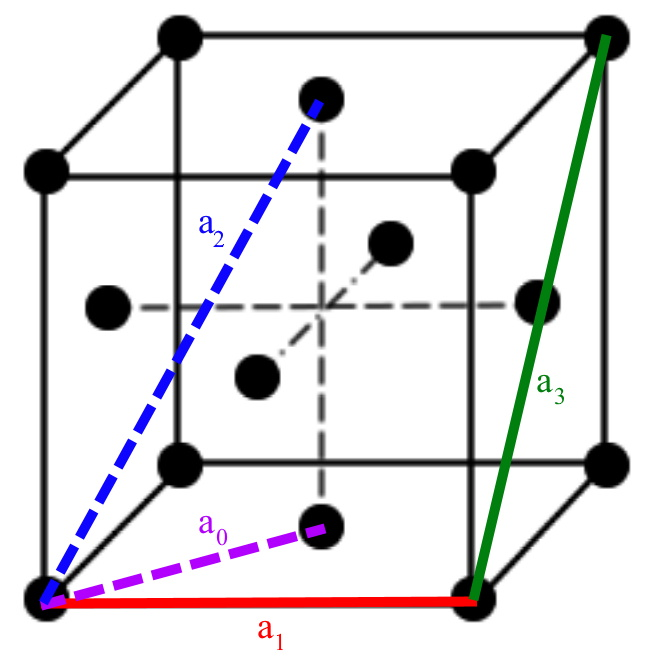
\includegraphics[width=0.4\linewidth]{Images/Lattice.jpg}
    \caption{FCC crystal structure with it's 4 shortest distances}
    \label{fig:Lattice}
\end{figure}\\
Where we write $a_1 = L/3$ with L = boxsize and express the other distances in function of $a_1$
\begin{equation}
    a_0 = \frac{a_1}{\sqrt{2}} = \frac{L}{3\sqrt{2}} \ \ \
    a_1  = L/3 \ \ \
    a_2 = a_1\sqrt{\frac{3}{2}} = \frac{L}{\sqrt{6}} \ \ \ a_3 = a_1\sqrt{2} = \frac{L\sqrt{2}}{3}
\end{equation}
The next closest distances would be the 3-dimensional diagonal however this distance would be $a_4 = a_1\sqrt{3} = \frac{L}{\sqrt{3}} > \frac{L}{2}$ and therefore it is not included.
\subsubsection{Pressure and Pair correlation values}
Rewriting the ideal gas law into a dimensionless form gives the following formula:
\begin{equation}
    PV=NTk_B \Rightarrow \Tilde{P} = \frac{P\sigma^3}{\epsilon} = \frac{N\Tilde{T}}{\Tilde{V}} = \Tilde{T}\Tilde{\rho}
\end{equation}
Using the values N=108,  $\Tilde{T}$ = 3.0 and $\Tilde{\rho}$ = 0.3 The pressure can be approximated to be $\Tilde{P} = 0.9$. Take note that this is not exact since the ideal gas law may or may not be a good approximation of the argon gas at these values.\\
\\
Looking at the relevant literature\cite{Johnson} for the gas ($\Tilde{T}$ = 3.0, $\Tilde{\rho}$ = 0.3) and liquid ($\Tilde{T}$ = 1.0, $\Tilde{\rho}$ = 0.8) phases, the following values can be found:
\begin{equation}
    \Tilde{P}_{gas} = 0.992 \pm 0.002 \ \ \ \ \Tilde{P}_{liquid} = 1.011 \pm 0.006
\end{equation}
The original paper of Verlet also has a similar pressure for the liquid for nearby initial conditions\cite{verlet1967}. Pressure values for the solid initial conditions were however not found by our search.\\
An attempt has been made to verify the pressure values for different initial conditions($\Tilde{\rho}$ = 0.9, $\Tilde{T}$ = 1.15 $\Rightarrow \Tilde{P}\approx$ 2.77) but in general the simulation kept underestimating these values compared to known results ($\Tilde{P} \approx $ 4.26)\cite{Johnson}. This discrepancy can probably be resolved due to the extra term introduced by Verlet to correct for the fact that the simulation is a finite system and neglects long range potential interactions.\cite{verlet1967}\\
\\
For the pair correlation values there should be 3 distinct characters for the different phases. As mentioned before in \eqref{Lattice} the atoms will be placed in a Lattice structure. While all our simulations start in this FCC initialisation, the solid state will remain in this structure throughout the simulations. The only exception will be an excitation allowing some slight movement of the atoms nearby their original position. Because of this the pair correlation function should exist of 4 distinct peaks for a solid. \\
\begin{figure}[!h]
    \centering
    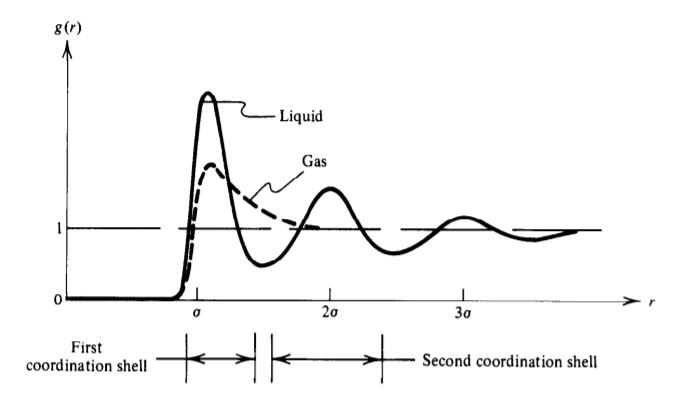
\includegraphics[width=0.63\linewidth]{Images/PairCorr.JPG}
    \caption{Structure of Pair Correlation Function for liquid and gas. Original image courtesy: Chandler David, Univeristy of California \cite{chandler}}
    \label{fig:my_label}
\end{figure}\\
\\
For liquids and gasses the pair correlation starts at 0 due to atomic overlap causing strong repulsion. After this both of their pair correlation functions will be centered around 1. The main difference is that the pair correlation for gas will start out as a single peak caused by Van der Waals interaction which decays to 1. While the pair correlation for liquid will consist of multiple peaks and pits around g(r) whose amplitude diminish at a further distance.\cite{chandler}

\subsubsection{Argon pressure-temperature phase diagram}
By converting the pressure and temperature units back to SI units by using the argon values for $\sigma = 3,405 $E-10 m and $\epsilon = 1,654 $E-21 J, one finds that $1 \Tilde{P} \approx 0.0419$ GPa and $1 \Tilde{T} \approx 100$ K. These conversions will then be used to check where the initial conditions of our simulation are.
\begin{figure}[!h]
    \centering
    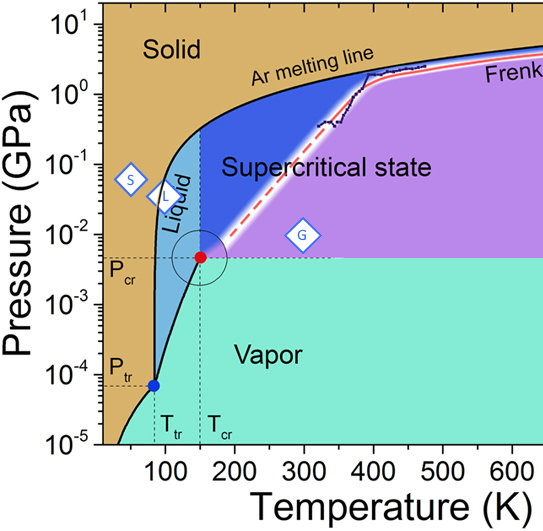
\includegraphics[width=0.5\linewidth]{Images/PhasesArgon.jpg}
    \caption{Simulation initial conditions for solid (S), liquid (L) and gas (G) denoted by the centre of the diamonds on the phase diagram. Original image courtesy: Bolmatov Dima et al. \cite{Frenkel1}}
    \label{fig:my_label}
\end{figure}\\
Where it seems obvious the initial conditions for gas and liquid correspond to the desired phase. For gas however it seems the simulation was performed in the supercritical fluid phase. However this supercritical fluid acts very similar to a gas when below the Frenkel line.\cite{Frenkel1}\cite{Frenkel2}
\newpage
\subsection{Pair Correlation Function}
\begin{wrapfigure}[14]{r}{8cm}
\raisebox{0pt}[\dimexpr\height-2\baselineskip\relax]{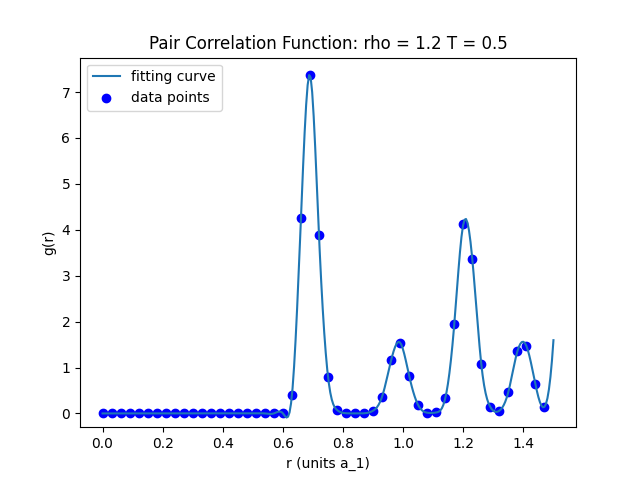
\includegraphics[width=8cm]{Data/pair_correlation_Solid.png}}
\caption{Pair Correlation function for a Solid}
\end{wrapfigure}\\
When plotting out the Pair Correlation Function it has been decided to rescale the x-axis to the side of a single cube lattice $a_1$ as described in Section \eqref{Lattice}.
This will make it much easier to check the corresponding solid state peaks as described.\\
\\
Looking at the figure on the right it is easy to check these peaks correspond with $r \in \{\frac{1}{\sqrt{2}}, 1, \frac{\sqrt{3}}{\sqrt{2}},\sqrt{2}\}$ just as predicted.\\
\\
The Pair Correlation Function for the liquid and gas below also follow the structure which has been described in theory and found back in different literature\cite{chandler}

\begin{figure}[!h]
    \begin{minipage}{.5\textwidth}
  \centering
  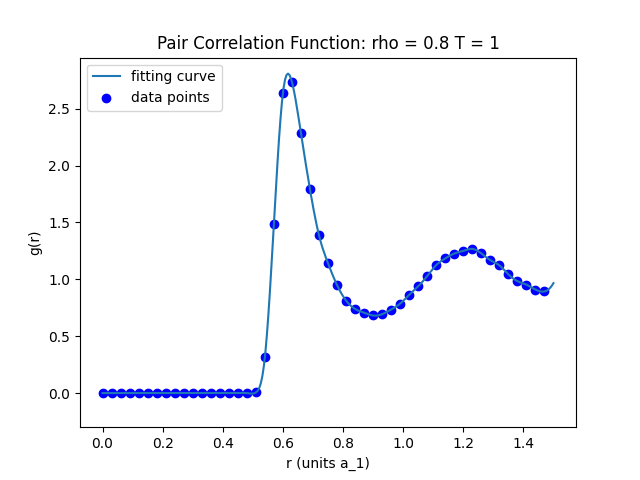
\includegraphics[width=1\linewidth]{Data/pair_correlation_Liquid.png}
\end{minipage}%
\begin{minipage}{.5\textwidth}
  \centering
  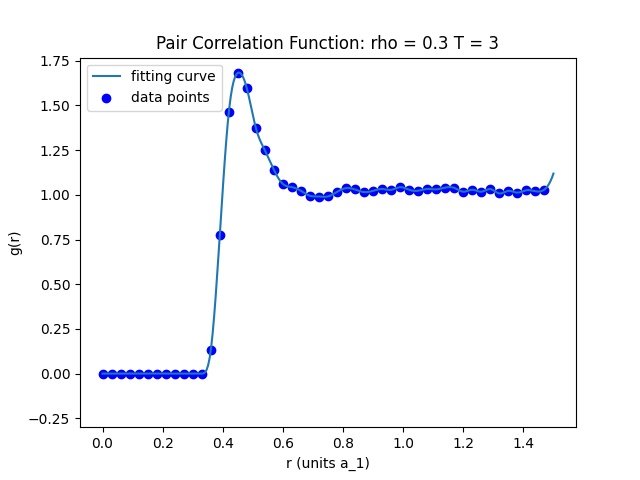
\includegraphics[width=1\linewidth]{Data/pair_correlation_Gas.png}

\end{minipage}
\caption{Left: Pair Correlation Function for liquid. Right: Pair Correlation Function for gas}
\end{figure}
The above Pair Correlation Functions have been made using 15000 time steps and generating a histogram every 50 steps after timestep 500.
\newpage
\subsection{Pressure}
The pressure of the system is calculated over 10000 timesteps and then averaged over 10 different runs.
\begin{table}[!htbp]
    \centering
    \begin{tabular}{c|c|c|c}
    \hline
    \multicolumn{4}{c}{Pressure}\\
    \hline
    Run & Solid & Liquid & Gas\\
    \hline
    1 & 8.6345 & 0.9475 & 0.9448\\
    \hline
    2 & 8.6433 & 0.9621 & 0.9700\\
    \hline
    3 & 8.6171 & 1.0073 & 0.9828\\
    \hline
    4 & 8.6038 & 1.0346 & 0.9900\\
    \hline
    5 & 8.5943 & 1.0292 & 0.9419\\
    \hline
    6 & 8.5666 & 1.1174 & 0.9652\\
    \hline
    7 & 8.5835 & 1.0937 & 0.9692\\
    \hline
    8 & 8.5721 & 1.0060 & 0.9733\\
    \hline
    9 & 8.5419 & 1.0501 & 0.9630\\
    \hline
    10 & 8.6356 & 0.9432 & 0.9420\\
    \hline
    Average & 8.5993 & 1.0191 & 0.9641\\
    \hline
    Standard deviation $\sigma_s$ & 0.0319 & 0.0557 & 0.0160\\
    \hline
    Standard error $SE$ & 0.0101 & 0.0176 & 0.0051\\
    \hline
    \end{tabular}
    \caption{Pressure simulation results.(Solid($\Tilde{\rho}$ = 1.2, $\Tilde{T}$ = 0.5), liquid($\Tilde{\rho}$ = 0.8, $\Tilde{T}$ = 1.0), gas($\Tilde{\rho}$ = 0.3, $\Tilde{T}$ = 3.0))}
    \label{tab:my_label}
\end{table}\\
The pressure value for the liquid and gas are closed to the values found in the literature \cite{Johnson} however we currently have no such value to compare the solid pressure with. There is however a slight difference between the calculated average and the known values. Increasing the amount of cubes in the system, making the system energy conserved when rescaling velocitiesmight help lower this difference with the known values.

\newpage
\section{Summary}
\label{Summary}
Molecular dynamics simulation is an effective approach to provide a vision into the a molecular level. Through Newtonian mechanics, it can solve equation of motion of a multi-particles system numerically. Our report is mainly based on Molecular dynamics to simulate Argon atoms with minimum image convention
of a FCC lattice consisting of $3\times3\times3$ cubes and compute the thermodynamic and statistical properties of different phase of argon(solid, liquid and gas).\par
Choosing Argon as our simulation object is because it is electrically neural and interact with no Coulomb force. When considering small displacements between nucleus and electron cloud, there exist attraction and repulsion. Thus, Lennard-Jones potential can describe these properties well.\par
%By using velocity Verlet algorithm, we start with initial conditions of density, temperature, fixed positions and Gaussian distributed velocities. Then we can calculate the positions and velocities of each particle for every time step. After all time steps, we compute system pressure and plot its pair correlation function.\par
Our main results is about the pressure and pair correlation function of different phases of Argon atoms. For pair correlation function, our plots fit well with theoretical prediction. It shows 4 peaks in solid phase. For liquid and gas, it tends to be 1 in late time steps. The main difference for gas and liquid is that liquid tends to have more peaks than gas. The pressure, for each phase, is calculated after 10000 time steps of simulation and averaged over 10 different runs. Our pressure value for each phase shows the agreement with the known experiment and simulation results. However for solid phase, our result has no simulation results to compare with. Moreover, it is likely that these results value can be improved by increasing the amount of cubes in the system and making the system energy conserved when rescaling velocities.\par
%----------------------------------------------------------------------------------------
%	BIBLIOGRAPHY
%----------------------------------------------------------------------------------------
\addcontentsline{toc}{section}{References}
\newpage
\bibliographystyle{unsrt}
\bibliography{bibfile}
%\begin{thebibliography}{99} % Bibliography - this is intentionally simple in this template
%\bibitem[Gramsa, 2005]{ArgonPhase}
%Gramsa, M., Stasickib, B., Toenniesc, J.P. (2005). `Production and characterization of micron-sized filaments of solid argon', {\em
%Review of Scientific Instruments}, \textbf{76}, 123904; https://doi.org/10.1063/1.2135277.
%\end{thebibliography}

%----------------------------------------------------------------------------------------
%	APPENDIX: THE CODE
%----------------------------------------------------------------------------------------





\end{document}